% Configurazione

\documentclass[a4paper]{article}
\usepackage{graphicx}
\usepackage[table,xcdraw]{xcolor}
\usepackage{titlesec}
\usepackage{hyperref}
\usepackage{fancyvrb}
\usepackage{amssymb}
\usepackage{geometry}
\usepackage{fancyhdr}
\usepackage{float}
\usepackage{longtable}
\usepackage[italian]{babel}
\usepackage{array}
\setcounter{section}{-1}
\newcolumntype{L}[1]{>{\raggedright\arraybackslash}p{#1}}
\newcolumntype{C}[1]{>{\centering\arraybackslash}p{#1}}
\newcolumntype{R}[1]{>{\raggedleft\arraybackslash}p{#1}}

\hypersetup{
    colorlinks=true,
    linkcolor=black,
    urlcolor=blue,
}

\geometry{
  top=30mm,
  bottom=30mm,
  left=30mm,
  right=30mm,
}

\pagestyle{fancy}
\lhead{}
\lfoot{Studio di Fattibilità}
\cfoot{}
\rfoot{\thepage}
\renewcommand{\headrulewidth}{0.4pt}
\renewcommand{\footrulewidth}{0.4pt}
\setlength{\headheight}{16pt}

\fancypagestyle{firstpage}{%
  \renewcommand{\headrulewidth}{0pt}%
  \renewcommand{\footrulewidth}{0pt}%
  \lfoot{}
  \rfoot{}
}

\graphicspath{ {immagini/} }
\definecolor{Rosso}{HTML}{B5121B}
\titleformat{\chapter}{\normalfont\huge}{\thechapter.}{20pt}{\huge\textbf}
\newcommand{\todo}[1]{\textcolor{red}{TODO: #1}}

% Variabili
\newcommand{\titolo}{Studio di Fattibilità}



% Struttura
\begin{document}
  \thispagestyle{firstpage}
  \begin{minipage}[]{0.90\textwidth}
  \begin{center}
    
\includegraphics[width=\textwidth]{Athesys.png}
  \end{center}
\end{minipage}

\bigskip

\begin{minipage}[]{0.7\textwidth}
  \begin{center}
    \hspace{2cm}
    \centering
    \textcolor{Rosso}{
      \textbf{Stage Athesys S.r.l.} \\
      \hspace{2cm}Laurea: Informatica \\
      \hspace{2cm}Anno Accademico: 2021/2022
    }
  \end{center}
\end{minipage}

\bigskip

\begin{minipage}[]{0.3\textwidth}
\end{minipage}
\begin{minipage}[]{0.7\textwidth}
  \centering
  \begin{center}
    \hspace{2cm}Studente: Emanuele Pase, mtr 1201250\\
    \hspace{2cm}Email: \texttt{emanuele.pase@studenti.unipd.it}
  \end{center}
\end{minipage}

\bigskip
\bigskip
\bigskip

  \begin{center}
  \Huge\textbf{\titolo}
\end{center}

\bigskip
\bigskip
\bigskip
  \newpage
  \tableofcontents
  \newpage
  %\listoftables
  %\newpage
  %\listoffigures

  % Capitoli
  \section{Introduzione}
FIDO Alliance è un associazione industriale lanciata nel Febbraio 2013 la cui missione è sviluppare e promuovere standard di autenticazione che riducano in maniera progressiva l'utilizzo di password. \\


\section{Architettura Metadata FIDO}
Per effettuare l'accesso alle risorse l'architettura FIDO si affida ai Metadata; essi servono per descrivere in maniera dettagliata la funzione di altri insiemi di dati e vengono utilizzati dal Relying Party (server che permettere l'accesso ad un'applicazione software) per autenticare e validare l'accesso ad una risorsa.\\

\'E possibile generalizzare i passi dell'autenticatore del metadata nel seguente modo:
\begin{itemize}
    \item L'authenticator vendor produce un'istruzione di metadati, che è codificata in UTF-8, la quale descrive le caratteristiche di un autenticatore.
    \item La dichiarazione dei metadati viene inviata alla FIDO Alliance nell'ambito del processo di certificazione FIDO. 
    \item Una relying party FIDO configura la propria politica di registrazione per consentire la registrazione di autenticatori che corrispondono a determinate caratteristiche.
    \item Il server FIDO invia un messaggio di richiesta di registrazione. Questo messaggio può contenere tale dichiarazione di politica.
    \item A seconda del protocollo FIDO utilizzato, l'applicazione della relying party o il client FIDO UAF riceve la dichiarazione della politica come parte del messaggio di richiesta e la elabora. Interroga gli autenticatori disponibili per le loro caratteristiche auto-segnalate e (con l'input dell'utente) seleziona un autenticatore che corrisponda alla politica, da registrare.
    \item Il client elabora e invia un messaggio di risposta di registrazione al server. Questo messaggio contiene un riferimento al modello dell'autenticatore e, facoltativamente, una firma effettuata con la chiave privata corrispondente alla chiave pubblica nel certificato di attestazione dell'autenticatore.
    \item Il server FIDO cerca l'istruzione di metadati per il particolare modello di autenticatore. Se la dichiarazione di metadati elenca uno o più certificati di attestazione, verifica che sia presente una firma di attestazione e che sia fatta con la chiave privata corrispondente a (1) uno dei certificati elencati in questa dichiarazione di metadati o (b) corrispondente alla chiave pubblica presente in un certificato che si concatena a uno dei certificati dell'emittente elencati nella dichiarazione dei Metadati dell'autenticatore.
    \item Il server FIDO verifica quindi che l'autenticatore soddisfi la politica di registrazione originariamente fornita in base alla sua dichiarazione di metadati autorevole. Ciò impedisce la registrazione di modelli di autenticatore imprevisti.
\end{itemize}

    \begin{center}
        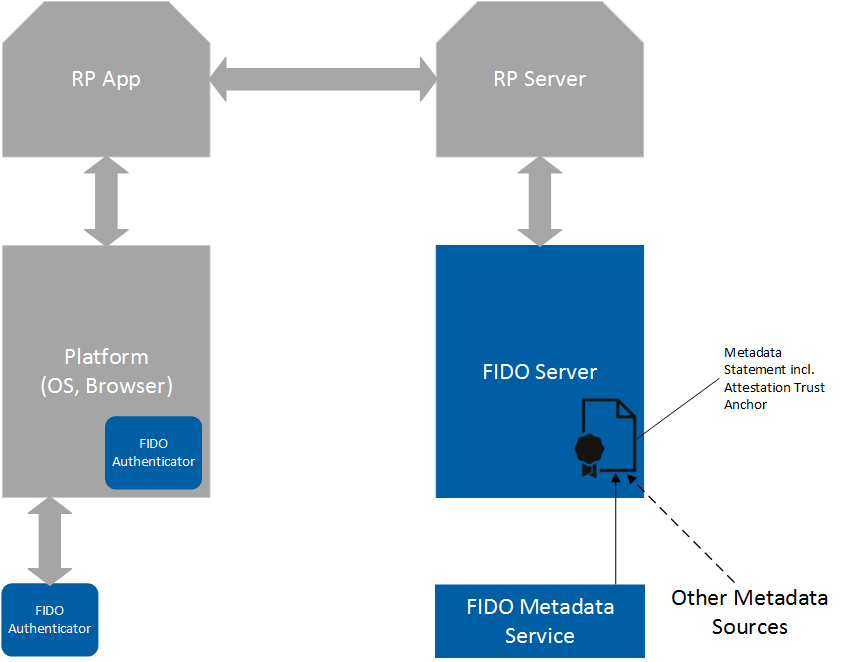
\includegraphics[width=0.7\textwidth]{fido-architecture.png}
    \end{center}

\section{Descrizione}


Lo scopo dello stage è quello di creare un convertitore per i Metadata FIDO, in modo che li trasformi dalla versione 2 alla versione più recente 3. \\

Per permettere tale conversione il programma necessiterà di funzionalità di supporto, come ad esempio:\begin{itemize}
    \item Parser per il metadata V2;
    \item Parser per il metadata V3;
    \item Logica per la conversione.
\end{itemize}
 
\section{Tecnologie Coinvolte}
Il programma verrà sviluppato utilizzando le seguenti tecnologie:\begin{itemize}
    \item Typescript, per qunto riguarda la stesura del codice;
    \item Node.js, per l'esecuzione dell'applicazione e dei test.
    \item Node modules principali utilizzati: \begin{itemize}
        \item debug: debugger javascript;
        \item jsdoc: documentazione;
        \item typescript: linguaggio utilizzato;
        \item ava: testing;
        \item fs: interazione con il sistema;
    \end{itemize}
\end{itemize}

\section{Vincoli}
I vincoli per la realizzazione del programma sono:\begin{itemize}
    \item Utilizzo di Typescript;
    \item Realizzazione parser Metadata V2;
    \item Realizzazione parser Metadata V3;
    \item Codifica test.
\end{itemize}

\section{Aspetti Positivi}
La realizzazione del programma permettere di certificare le funzionalità FIDO implementate dall'azienda \textit{Athesys S.r.l.} sfruttando una libreria esterna. La necessità di creare il programma nasce dal fatto che tale libreria accetta solamente Metadata della versione 2, quando l'infrastruttura aziendale è basata sulla versione successiva.

\section{Aspetti Critici}
La realizzazione del programma permette di verificare l'infrastruttura certificandola con la versione precedente del Metadata, ciò significa che alcune nuove funzionalità introdotte con la nuova versione non potranno essere testate e certificate per il momento.

\section{Conclusioni}
Possiamo dunque comprendere che, per semplificare l'interoperabilità e l'integrazione delle funzionalità FIDO, sia importante creare un programma che permetta di convertire i metadata da una versione all'altra. 
\end{document}
